%%%%%%%%%%%%%%%%%%%%%%%%%%%%%%%%%%%%%%%%%%%%%%%%%%%%%%%%%%%%%%%%%%%%%%
% Problem statement
\begin{statement}[
  problempoints=110,
  timelimit=3 sekunde,
  memorylimit=512 MiB,
]{Checker}

``\textit{...fool me once, shame on — shame on you. Fool me — you can't get fooled again.}''
-- W.

U ovom zadatku promatramo pravilne $N$-terokute kojima su stranice obojene u
tri boje, a vrhovi označeni prirodnim brojevima u smjeru kazaljke na satu.
\textit{Triangulacija} je podjela mnogokuta na trokute unutarnjim
dijagonalama takva da dijagonale nemaju zajedničkih točaka osim vrhova
mnogokuta te ne sijeku stranice mnogokuta osim u vrhovima mnogokuta.
Naravno, u ovom zadatku i svaka će dijagonala biti obojena u jednu od tri
boje.

Triangulacija je \textit{domoljubna} ako za svaki od $N-2$ trokuta vrijedi da
su mu sve tri stranice različite boje. Vaš je zadatak odrediti čine li
dijagonale triangulaciju te je li ta triangulacija domoljubna.

%%%%%%%%%%%%%%%%%%%%%%%%%%%%%%%%%%%%%%%%%%%%%%%%%%%%%%%%%%%%%%%%%%%%%%
% Input
\subsection*{Ulazni podaci}
U prvom je retku redni broj podzadatka kojem pripada testni primjer
(vidi tablicu u poglavlju o bodovanju). Ako vaše rješenje ne mari za podzadatke,
samo ga učitajte i ignorirajte.

U drugom je retku prirodan broj $N$ iz teksta zadatka.

U trećem je retku $N$-teroznamenkasti broj čije znamenke predstavljaju boje
stranica $N$-terokuta u smjeru kazaljke na satu. Odnosno, prva znamenka
predstavlja boju stranice $(1,2)$, druga znamenka boju stranice $(2,3)$ i tako
sve do $N$-te znamenke koja predstavlja boju stranice $(N, 1)$. Dakako, boje su
označene znamenkama $1$, $2$ i $3$.

U svakom od sljedećih $N-3$ redaka nalazi se po jedna dijagonala u obliku
$X$ $Y$ $C$, gdje su $X$ i $Y$ vrhovi dijagonale, a $C$ boja
$(1 \le X, Y \le N, 1 \le C \le 3)$. Svaki redak će opisivati validnu
dijagonalu, odnosno vrhovi $X$ i $Y$ neće biti ni isti ni susjedni.

%%%%%%%%%%%%%%%%%%%%%%%%%%%%%%%%%%%%%%%%%%%%%%%%%%%%%%%%%%%%%%%%%%%%%%
% Output
\subsection*{Izlazni podaci}
Ako zadane dijagonale ne čine triangulaciju, ispišite
\texttt{"neispravna triangulacija"} (bez navodnika).

Ako pak dijagonale čine triangulaciju, no ona nije domoljubna, ispišite
\texttt{"neispravno bojenje"} (bez navodnika).

Ako dijagonale čine domoljubnu triangulaciju, ispišite \texttt{"tocno"}
(bez navodnika).

%%%%%%%%%%%%%%%%%%%%%%%%%%%%%%%%%%%%%%%%%%%%%%%%%%%%%%%%%%%%%%%%%%%%%%
% Scoring
\subsection*{Bodovanje}
{\renewcommand{\arraystretch}{1.4}
  \setlength{\tabcolsep}{6pt}
  \begin{tabular}{ccl}
 Podzadatak & Broj bodova & Ograničenja \\ \midrule
  1 & 12 & $4 \le N \le 300$ \\
  2 & 17 & $4 \le N \le 2000$ \\
    3 & 23 & $4 \le N \le 2\cdot10^5$, odgovor je \texttt{neispravna triangulacija} ili \texttt{tocno} \\
    4 & 23 & $4 \le N \le 2\cdot10^5$, odgovor je \texttt{neispravno bojenje} ili \texttt{tocno} \\
  5 & 35 & $4 \le N \le 2\cdot10^5$
\end{tabular}}

Za razliku od zadatka \textit{Trobojnica}, ako vaš program točno ispisuje prvi redak u
svakom testnom primjeru nekog podzadatka, osvojit će $100\%$ bodova predviđenih
za taj podzadatak.

%%%%%%%%%%%%%%%%%%%%%%%%%%%%%%%%%%%%%%%%%%%%%%%%%%%%%%%%%%%%%%%%%%%%%%
% Examples
\subsection*{Probni primjeri}
\begin{tabularx}{\textwidth}{X'X'X}
\sampleinputs{test/checker.dummy.in.1}{test/checker.dummy.out.1} &
\sampleinputs{test/checker.dummy.in.2}{test/checker.dummy.out.2} &
\sampleinputs{test/checker.dummy.in.3}{test/checker.dummy.out.3}
\end{tabularx}


\textbf{Pojašnjena probnih primjera:}

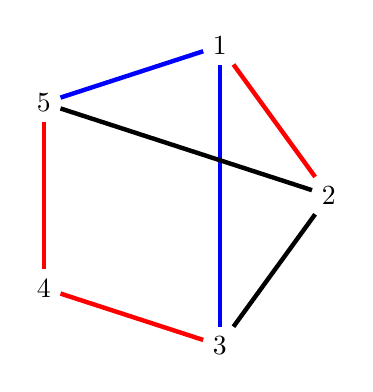
\begin{tikzpicture}
    \def\r{2}

    \node(1) at (1*360/5:\r) {1};
    \node(2) at (0*360/5:\r) {2};
    \node(3) at (4*360/5:\r) {3};
    \node(4) at (3*360/5:\r) {4};
    \node(5) at (2*360/5:\r) {5};

    \draw [ultra thick, red]   (1) -- (2);
    \draw [ultra thick, black] (2) -- (3);
    \draw [ultra thick, red]   (3) -- (4);
    \draw [ultra thick, red]   (4) -- (5);
    \draw [ultra thick, blue]  (5) -- (1);

    \draw [ultra thick, blue]  (1) -- (3);
    \draw [ultra thick, black] (2) -- (5);
\end{tikzpicture}
\hspace{30pt}
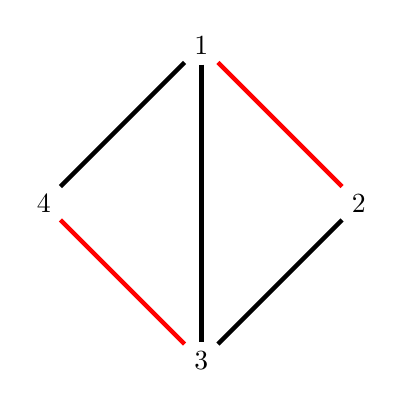
\begin{tikzpicture}
    \def\r{2}

    \node(1) at (1*360/4:\r) {1};
    \node(2) at (0*360/4:\r) {2};
    \node(3) at (3*360/4:\r) {3};
    \node(4) at (2*360/4:\r) {4};

    \draw [ultra thick, red]   (1) -- (2);
    \draw [ultra thick, black] (2) -- (3);
    \draw [ultra thick, red]   (3) -- (4);
    \draw [ultra thick, black] (4) -- (1);

    \draw [ultra thick, black] (1) -- (3);
\end{tikzpicture}
\hspace{30pt}
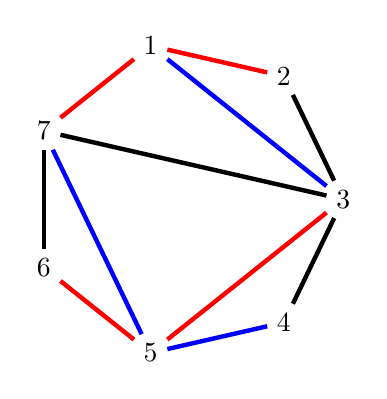
\begin{tikzpicture}
    \def\r{2}

    \node(1) at (2*360/7:\r) {1};
    \node(2) at (1*360/7:\r) {2};
    \node(3) at (0*360/7:\r) {3};
    \node(4) at (6*360/7:\r) {4};
    \node(5) at (5*360/7:\r) {5};
    \node(6) at (4*360/7:\r) {6};
    \node(7) at (3*360/7:\r) {7};

    \draw [ultra thick, red]   (1) -- (2);
    \draw [ultra thick, black] (2) -- (3);
    \draw [ultra thick, black] (3) -- (4);
    \draw [ultra thick, blue]  (4) -- (5);
    \draw [ultra thick, red]   (5) -- (6);
    \draw [ultra thick, black] (6) -- (7);
    \draw [ultra thick, red]   (7) -- (1);

    \draw [ultra thick, blue]  (1) -- (3);
    \draw [ultra thick, red]   (3) -- (5);
    \draw [ultra thick, blue]  (5) -- (7);
    \draw [ultra thick, black] (7) -- (3);
\end{tikzpicture}

%%%%%%%%%%%%%%%%%%%%%%%%%%%%%%%%%%%%%%%%%%%%%%%%%%%%%%%%%%%%%%%%%%%%%%
% We're done
\end{statement}

%%% Local Variables:
%%% mode: latex
%%% mode: flyspell
%%% ispell-local-dictionary: "croatian"
%%% TeX-master: "../hio.tex"
%%% End:
